\documentclass[12pt,]{article}
\usepackage{lmodern}
\usepackage{amssymb,amsmath}
\usepackage{ifxetex,ifluatex}
\usepackage{fixltx2e} % provides \textsubscript
\ifnum 0\ifxetex 1\fi\ifluatex 1\fi=0 % if pdftex
  \usepackage[T1]{fontenc}
  \usepackage[utf8]{inputenc}
\else % if luatex or xelatex
  \ifxetex
    \usepackage{mathspec}
  \else
    \usepackage{fontspec}
  \fi
  \defaultfontfeatures{Ligatures=TeX,Scale=MatchLowercase}
\fi
% use upquote if available, for straight quotes in verbatim environments
\IfFileExists{upquote.sty}{\usepackage{upquote}}{}
% use microtype if available
\IfFileExists{microtype.sty}{%
\usepackage{microtype}
\UseMicrotypeSet[protrusion]{basicmath} % disable protrusion for tt fonts
}{}
\usepackage[margin=0.50in]{geometry}
\usepackage{hyperref}
\hypersetup{unicode=true,
            pdftitle={COVID-19 subject J37GK},
            pdfborder={0 0 0},
            breaklinks=true}
\urlstyle{same}  % don't use monospace font for urls
\usepackage{graphicx,grffile}
\makeatletter
\def\maxwidth{\ifdim\Gin@nat@width>\linewidth\linewidth\else\Gin@nat@width\fi}
\def\maxheight{\ifdim\Gin@nat@height>\textheight\textheight\else\Gin@nat@height\fi}
\makeatother
% Scale images if necessary, so that they will not overflow the page
% margins by default, and it is still possible to overwrite the defaults
% using explicit options in \includegraphics[width, height, ...]{}
\setkeys{Gin}{width=\maxwidth,height=\maxheight,keepaspectratio}
\IfFileExists{parskip.sty}{%
\usepackage{parskip}
}{% else
\setlength{\parindent}{0pt}
\setlength{\parskip}{6pt plus 2pt minus 1pt}
}
\setlength{\emergencystretch}{3em}  % prevent overfull lines
\providecommand{\tightlist}{%
  \setlength{\itemsep}{0pt}\setlength{\parskip}{0pt}}
\setcounter{secnumdepth}{0}

%%% Use protect on footnotes to avoid problems with footnotes in titles
\let\rmarkdownfootnote\footnote%
\def\footnote{\protect\rmarkdownfootnote}

%%% Change title format to be more compact
\usepackage{titling}

% Create subtitle command for use in maketitle
\newcommand{\subtitle}[1]{
  \posttitle{
    \begin{center}\large#1\end{center}
    }
}

\setlength{\droptitle}{-2em}

  \title{COVID-19 subject J37GK}
    \pretitle{\vspace{\droptitle}\centering\huge}
  \posttitle{\par}
    \author{}
    \preauthor{}\postauthor{}
      \predate{\centering\large\emph}
  \postdate{\par}
    \date{2020-09-14}

\usepackage{pdflscape}
\newcommand{\blandscape}{\begin{landscape}}
\newcommand{\elandscape}{\end{landscape}}
\usepackage{pdfpages}
\usepackage{booktabs}
\usepackage{makecell}
\usepackage{float}

\begin{document}
\maketitle

The table below provides a summary of subject samples for which
sequencing data is available.\\
The experiments column shows the number of sequencing experiments
performed for each specimen.\\
Experiment specific analyses are shown at the end of this report. The
code base for this analysis can be found
(\href{https://github.com/everettJK/SARS-CoV-2-Philadelphia}{here}).

\vspace{0.5cm}

\small
Table 1. Sample summary. \normalsize

\begin{table}[H]
\centering
\resizebox{\linewidth}{!}{
\begin{tabular}{ccc>{\centering\arraybackslash}p{2cm}c>{\centering\arraybackslash}p{3cm}>{\centering\arraybackslash}p{3cm}>{\centering\arraybackslash}p{5cm}}
\toprule
Experiment & Type & Input genomes & Sample type & Sample date & Largest contig (KD) & Reference read
coverage & Reference read
coverage (>= 5 reads)\\
\midrule
VSP9991-1 & single experiment & NA & WaterControl & 2020-06-13 & NA & 4.9\% & 2.4\%\\
\bottomrule
\end{tabular}}
\end{table}

\newpage

\subsubsection{Variants shared across
samples}\label{variants-shared-across-samples}

The heat map below shows how variants (reference genome USA-WA1-2020)
are shared across subject samples where the percent variance is colored.
Variants are called if a variant position is covered by 5 for more
reads, the alternative base is found in \textgreater{} 50\% of read
pairs and the variant yields a PHRED score \textgreater{} 20. Gray tiles
denote positions where the variant was not the major variant or no
variants were found. The relative base compositions of each experiment
used to calculate tiles are shown in the following plot where the total
number of position reads are shown atop of each plot.

\vspace{0.5cm}

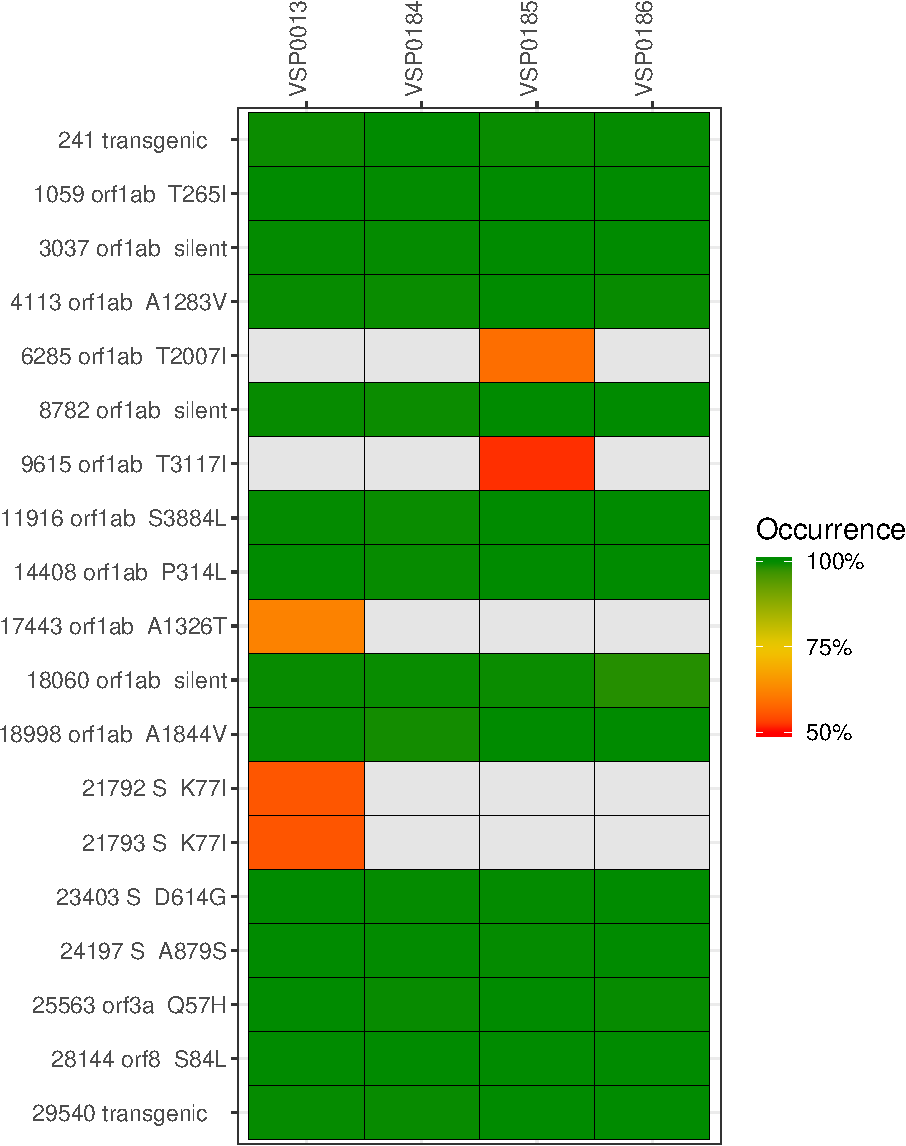
\includegraphics{summaries/patientReports/J37GK_files/figure-latex/unnamed-chunk-2-1.pdf}

\newpage

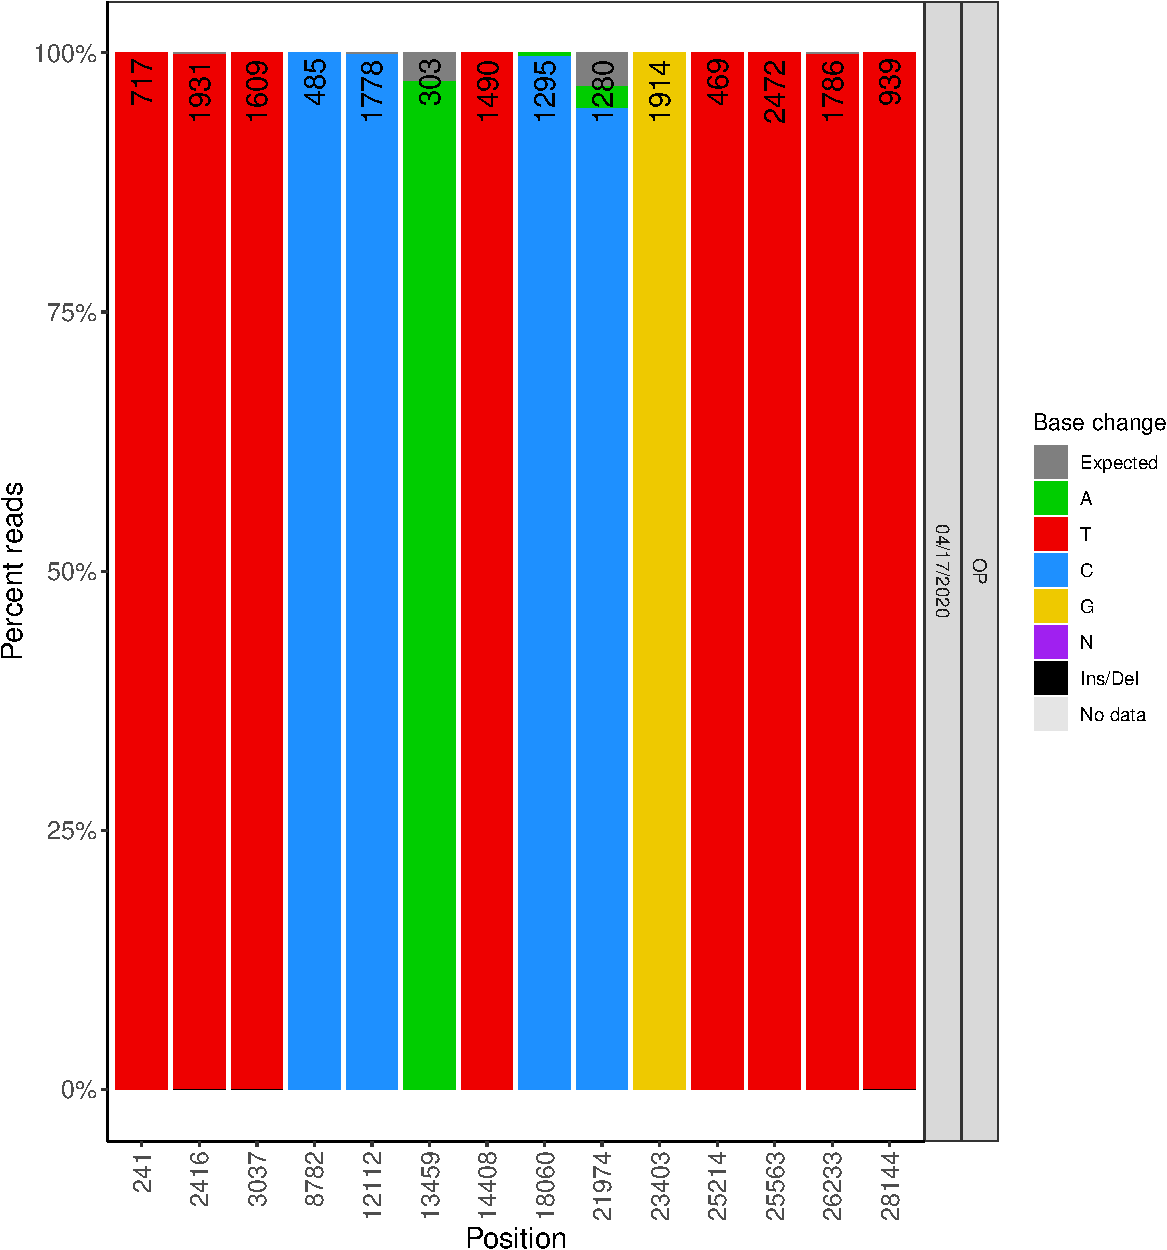
\includegraphics{summaries/patientReports/J37GK_files/figure-latex/unnamed-chunk-3-1.pdf}

\newpage

\subsection{Analyses of individual experiments and composite
results.}\label{analyses-of-individual-experiments-and-composite-results.}

\subsubsection{VSP9991-1 \textbar{} 2020-06-13 \textbar{} WaterControl
\textbar{} J37GK \textbar{} genomes \textbar{} single
experiment}\label{vsp9991-1-2020-06-13-watercontrol-j37gk-genomes-single-experiment}

The plot below shows the number of reads covering each nucleotide
position in the reference genome. Variants are shown as colored dots
along the bottom of the plot and are color coded according by variant
types: gray - transgenic, green - silent, gold - missense, red -
nonsense, black - indel.

\vspace{0.23cm}

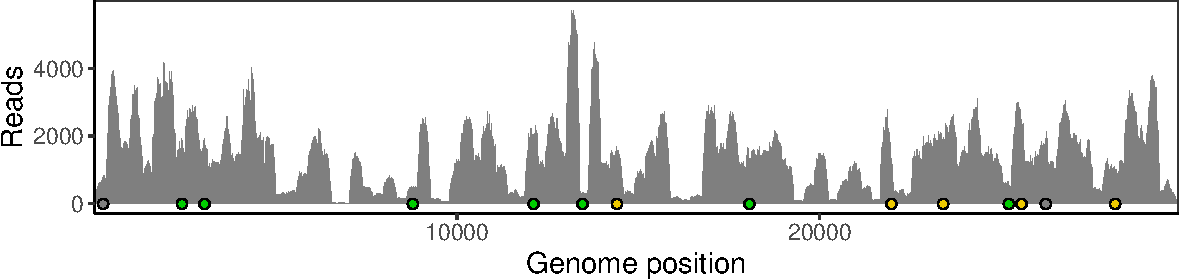
\includegraphics{summaries/patientReports/J37GK_files/figure-latex/unnamed-chunk-4-1.pdf}

\vspace{0.35cm}

\vspace{0.25cm} Excerpt from plot above focusing on reads coverage from
0 to 50 NT.

\vspace{0.25cm}

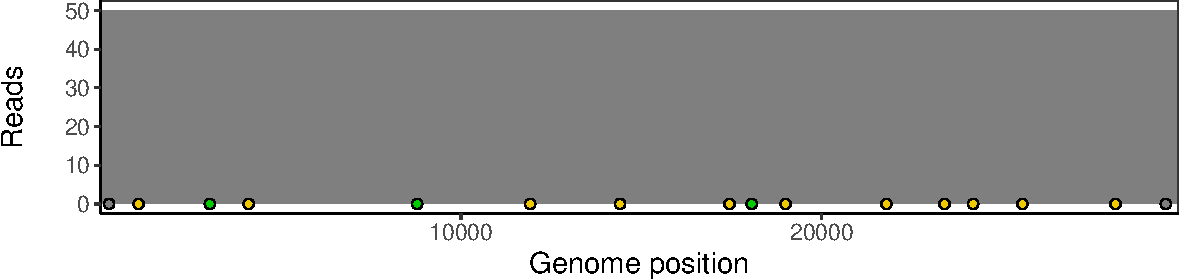
\includegraphics{summaries/patientReports/J37GK_files/figure-latex/unnamed-chunk-4-2.pdf}

\vspace{0.50cm}

\subsection{No contig data available.}\label{no-contig-data-available.}

\vspace{0.50cm}

\newpage

\newpage


\end{document}
